\section{Bestrahlungsplanung}
\label{sec:Bestrahlungsplanung}
Das PTV ist in den CT-Daten bereits eingezeichnet und als nächstes ist die Kontur des Schädels als Body-Struktur eingezeichnet worden.
Risikoorgane bei dieser Bestrahlung sind die Linsen und diese werden auch in den CT-Daten eingezeichnet. Außerdem werden noch die gesamten Augen
und die Knochen eingezeichnet.
Für die Bestrahlungsplanung werden zwei opponierende Felder
mit einer Gewichtung von 0.5 verwendet. Die beiden Felder haben eine Größe von $\SI{5,9}{\centi\meter}$ x $\SI{5,7}{\centi\meter}$.
Das erste Feld hat eine Gantry-Rotation von $90^\circ$ und das zweite eine Gantry-Rotation von $270^\circ$.
Der Bestrahlungsplan wird auf \enquote{$\SI{100}{\percent}$ target mean} normiert. Für eine Schonung der Risikoorganen als auch des Gehirns werden
MLCs verwendet, die an das PTV angepasst werden. Die einstellungen der MLCs sind in den Abbildungen \ref{fig:mlcfeld1} und \ref{fig:mlcfeld2} zu sehen.
Damit die Linsen geschont werden, wurden die Lamellen der MLCs in dem Bereich der Augenlinsen manuell angepasst.

\begin{figure}[h]
	\centering
	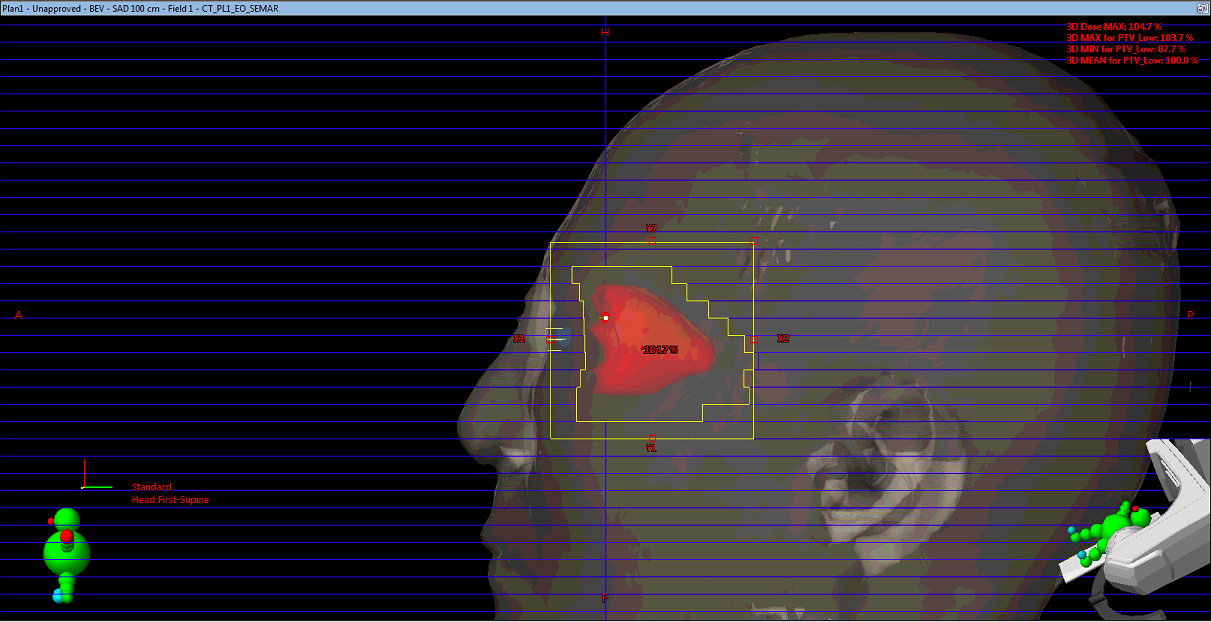
\includegraphics[width=0.8\linewidth]{Bilder/MLC_Feld1}
	\caption{Zu sehen ist die Darstellung der Lamellen beim MLC. Es handelt sich um das Feld bei $90^\circ$.}
	\label{fig:mlcfeld1}
\end{figure}

\begin{figure}[h]
	\centering
	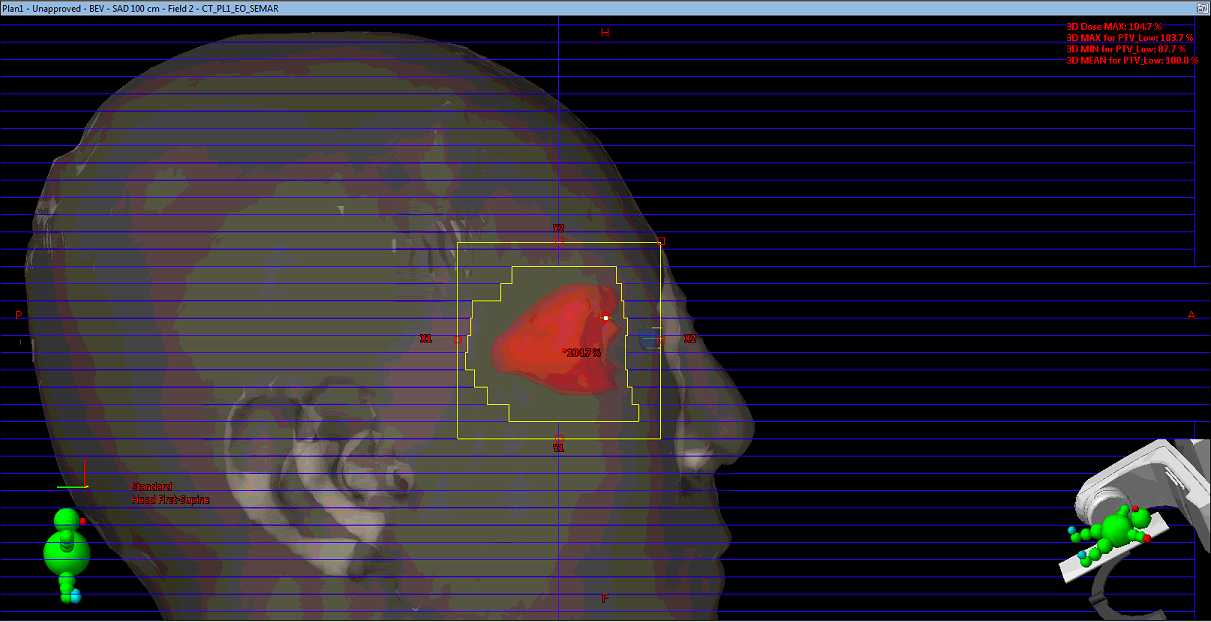
\includegraphics[width=0.8\linewidth]{Bilder/MLC_Feld2}
	\caption{Zu sehen ist die Darstellung der Lamellen beim MLC. Es handelt sich um das Feld bei $270^\circ$.}
	\label{fig:mlcfeld2}
\end{figure}
